\section{GPU}

One of the goals of this thesis is to analyze the possibilities of accelerating cross-correlation algorithm, described in chapter \ref{sec:cross-corr}, using Graphics processing unit (GPU). This chapter first provides short introduction into the history of the GPU \ref{sec:gpu_history}, which helps us in the section \ref{sec:cuda} to better understand the possibilities and restrictions of the CUDA environment.


\subsection{History of the GPU}
\label{sec:gpu_history}
The acronym GPU was first coined by Sony in 1994 with the launch of the PS1 for the Sony GPU, at the time referring to geometry processing unit. Later, this acronym was transformed by NVIDIA % TODO: Link under the line
 into the graphics processing unit we know today with the launch of GeForce 256 in 1999, as described by \citep{gpuacro} in his article "Is it Time to Rename the GPU?". 
As the name suggests, GPUs were designed as co-processors, or separate devices, for offloading the computationally expensive work of transformation, clipping, lighting, rasterization and texturing of 3D geometry. Apart from freeing the CPU processing power that would otherwise be taken up by these operations, the main advantage of GPUs is that the operations are implemented in hardware, allowing for much higher throughput. 

Whereas CPUs are designed for task parallelism and low latency with complex flow control, the massively data parallel task of 3D geometry processing led to GPUs being designed to maximize throughput. % TODO?: \citep{paper:gpu_history}

First generations of GPUs had what was called a "fixed function pipeline", which can be seen on the figure \ref{fig:gpu_fixed_pipeline}. The operations done for each vertex of the 3D geometry and each fragment after rasterization were either completely fixed, represented by the blue rectangles in the figure \ref{fig:gpu_fixed_pipeline}, or only configurable by providing a set of matrices and textures to the pipeline, represented by yellow rectangles in the figure, as described in the book "Programming Massively Parallel Processors" by \citep{book:paraproc}. These fixed pipelines were accessible through several APIs, most commonly the OpenGL and Direct3D APIs.

\begin{figure}[h]
	\centering
	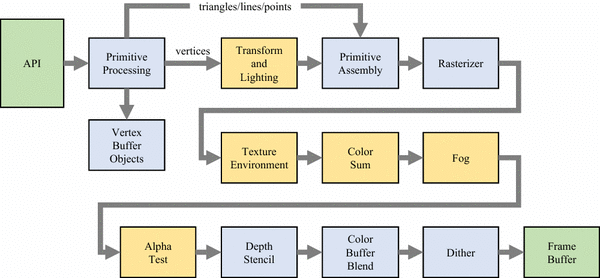
\includegraphics[width=0.8\textwidth]{gpu_fixed_pipeline.png}
	\caption{Fixed function GPU pipeline.}
	\label{fig:gpu_fixed_pipeline}
\end{figure}

With DirectX 8 and OpenGL vertex shader extensions  came the first step to GPU computations, the programmable vertex shader, as described by \citep[28]{book:paraproc}. 
% TODO: Describie what vertex shader is

In 2002 came the extension to programmable fragment shader, which at this point had a separate processor design due to the massive amount of fragments that have to be manipulated compared to the amount of vertices processed by the vertex shader. The change to the pipeline can be seen when comparing figure \ref{fig:gpu_fixed_pipeline} to figure \ref{fig:gpu_programmable_pipeline}. In the figure \ref{fig:gpu_programmable_pipeline}, all previously configurable stages were replaced by the two programmable shader stages.

\begin{figure}[h]
	\centering
	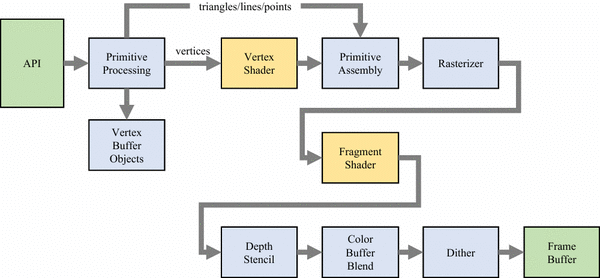
\includegraphics[width=0.8\textwidth]{gpu_programmable_pipeline.png}
	\caption{Programmable GPU pipeline.}
	\label{fig:gpu_programmable_pipeline}
\end{figure}

With additional shader stages such as geometry shaders, tesselation shaders etc., and the need for more processing power in each stage, the following generations of GPUs such as GeForce 8800 unified the underlying hardware for these stages into a single hardware package which is reused by all the shader stages as described by \citep[33]{book:paraproc}. This paved the way for the use of this hardware package for more than just processing graphics, leading to the development of general purpose GPUs, described in the section \ref{sec:gpgpu}. 

As said by \citep{paper:accelerator}: "Shader programs are strict SIMD programs." Single instruction multiple data (SIMD) is a parallel programming paradigm in Flynn's taxonomy where the same operation is applied to multiple elements of a dataset at once. In the case of shaders, the same operation can be applied to all elements in the dataset at once. This data independence as the dominating application characteristic is a key difference between the design assumptions for GPUs and CPUs. As these operations work predominantly with floating point data, this gives GPUs unparalleled throughput when processing this type of data.

Additionally, as said by \citep{book:paraproc}, common rendering algorithms perform a single pass over input primitives, be it vertices of 3D geometry or fragments created by rasterization, which leads to highly coherent access to memory and other resources. As a result, the algorithms exhibit excellent spatial locality for memory access, alleviating the need for large data caches and instead leaning more heavily on large memory bandwidth and many parallel processing units.

\subsubsection{GPGPU}
\label{sec:gpgpu}
With the advent of programmable shaders, problems other than 3D graphics could be solved using GPUs. This was the beginning of General-purpose computing on Graphics Processing Units (GPGPU).

In these initial stages, the problems had to be reformulated in terms of graphical primitives so that existing APIs such as OpenGL and DirectX could be used to run pixel shader (also known as fragment shader) code for solving the problem. \citep{paper:accelerator}. Pixel shader environment is very restrictive, requiring complete independence of the operations on each input element, limiting the amount of registers available and in some shaders allowing only a single value to be computed per pixel shader run. % TODO: More

To simplify the complex process of reformulating the problem into the terms of computer graphics, frameworks such as Accelerator by \citep{paper:accelerator} and Sh % TODO: Cite 
were created. These abstract away some of the limitations of the underlying pixel shaders by providing a simplified API, such as data-parallel arrays in the case of Accelerator, and using Just-In-Time compilation, transforming input data into textures and generating pixel shaders to run the requested operations on the input textures. 

Even with the use of these frameworks, the limitations of the underlying graphics APIs and infrastructure limited the scope of problems that could be solved using the computational power of GPUs. 

To remove these limitations and restrictions, tools such as CUDA, ATI FireStream and OpenCL were introduced. Designed by the GPU manufacturers themselves, these tools allow users to bypass the step of transforming the problem to graphics concepts and access the full hardware capability and parallelism directly. From these, the most prevalent today is CUDA, which will be used in our work and will be described in the following section \ref{sec:cuda}.
 

\subsection{CUDA}
\label{sec:cuda}

Compute Unified Device Architecture, better known by its acronym CUDA, introduced in 2006, is a "general purpose parallel computing platform and programming model" as described by \citep{site:cuda}, allowing users to utilize NVIDIA GPUs to solve complex computational problems.


CUDA presents a programming model consisting of abstractions of thread groups, shared memories and barrier synchronizations, allowing transparent scaling with the number of processing cores just as 3D graphics applications do.

CUDA code is split between "host" code and "device" code. Host code is the code running on the CPU, working with operating memory and accessing the operating system the same way any other non-CUDA code would. Device code on the other hand runs on one or more "devices". Each device corresponds to a single GPU, or in newer versions to one or more slices of a GPU. CUDA code is described in more detail in the \ref{sec:cuda_cpp} section.
% TODO: Describe Ampere and MIG https://docs.nvidia.com/datacenter/tesla/mig-user-guide/index.html

One of the distinguishing features of device code is that it runs concurrently with the host code, as can be seen on the time diagram \ref{fig:concurrent_device}. This allows the CPU to do other tasks while devices run the device code.

Another important feature is the device memory, which is separate both from the device memory of each other device and from the host system memory. Data has to be explicitly transferred between the host operating memory and the device memory. This transfer can either be done manually using the CUDA API in the host code, or automatically behind the scenes by allocating the memory using the CUDA API with the correct flags. CUDA memory handling is described in more detail in the section \ref{sec:memory_hierarchy}.

% TODO: More on Host and device

\subsubsection{Compute capability}
\label{sec:compute_capability}
% TODO: Compute capability table
Whereas versions of CUDA specify the version of the CUDA software platform, i.e. the abstractions and tools used to create the CUDA programs, Compute capability identifies features supported by the hardware of given GPU. Most often a release of new major CUDA version coincides with the release of new Compute capability GPUs, allowing access to the new capabilities provided by the hardware. Each CUDA version has minimal supported Compute capability, which identifies the minimal hardware capabilities the CUDA compiler and CUDA runtime require to emulate the hardware capabilities of the Compute capability the CUDA version was released with.

CUDA versions are forward compatible with newer Compute capabilities than the one the CUDA version was released with. This means that any CUDA code can run on the newest GPUs, albeit without using the newer capabilities of the hardware. 

Good analogy for this is the version of C\# as a language and the .NET runtime, where version of C\# corresponds to the CUDA version, and version of the .NET runtime corresponds to Compute capability. This analogy is aided by the fact that CUDA is by its nature JIT compiled, same as C\#, as described in the section \ref{sec:cuda_compilation}. Even though it is designed for JIT compilation, it often is compiled ahead of time.



\subsubsection{SIMT}
\label{sec:simt}
The single instruction, multiple threads (SIMT) execution model is the underpinning abstraction of the CUDA platform. The SIMT execution model is very similar to SIMD in that single instruction controls multiple processing elements as described by \citep{site:cuda} in CUDA C++ programming guide. The main difference is that SIMT code specifies the behavior of a single thread, whereas SIMD code specifies the behavior of all the lanes based on the width of the SIMD instructions. SIMT code can thus run data-parallel coordinated code just as SIMD would, but it can also branch independently in each thread.

Threads in the SIMT execution model of CUDA are scheduled in groups of 32, called warps. When targeting Compute capabilities before Volta, all threads of a warp share instruction and stack pointer, thus executing in lockstep. Independent branching is achieved by executing all code in all branches by all threads of the warp and masking the threads which are not supposed to execute the given code branch, as can be seen on the figure \ref{fig:thread_divergence_old}. We call this that the threads diverged. After the diverging branches are executed, the threads are reconverged and continue executing in lockstep.  %This is one of the hints for the internal width of the vector units in the Streaming Multiprocessor as described in the section \ref{sec:sm}, which hints at internal width of 1024 bits for the vector units. 

In Compute capabilities after Volta, each thread has its own instruction pointer and stack pointer, allowing independent branching and requiring explicit synchronization of threads in a warp as can be seen on the figure \ref{fig:thread_divergence_new}. This change allows finer-grained synchronization and cooperation between threads, as well as finer-grained scheduling in sub-warp granularity. Before, divergent threads in the same warp could not signal each other or cooperate as they could with threads from different warps in the same block, which presented an inconsistency in the programming model. This required programmers to use lock-free or warp-aware algorithms.
The new execution model allows the GPU to yield execution of any thread, allowing threads to wait for data produced by another thread regardless of the warp the producer is in. Threads in a single warp are still executed in lockstep where possible to preserve the high through of the previous model, but where needed the threads can diverge and reconverge in sub-warp granularity. This allows programmers to use starvation-free algorithms with standard locking.
% TODO: Cite https://developer.nvidia.com/blog/inside-volta/

\begin{figure}[h]
	\centering
	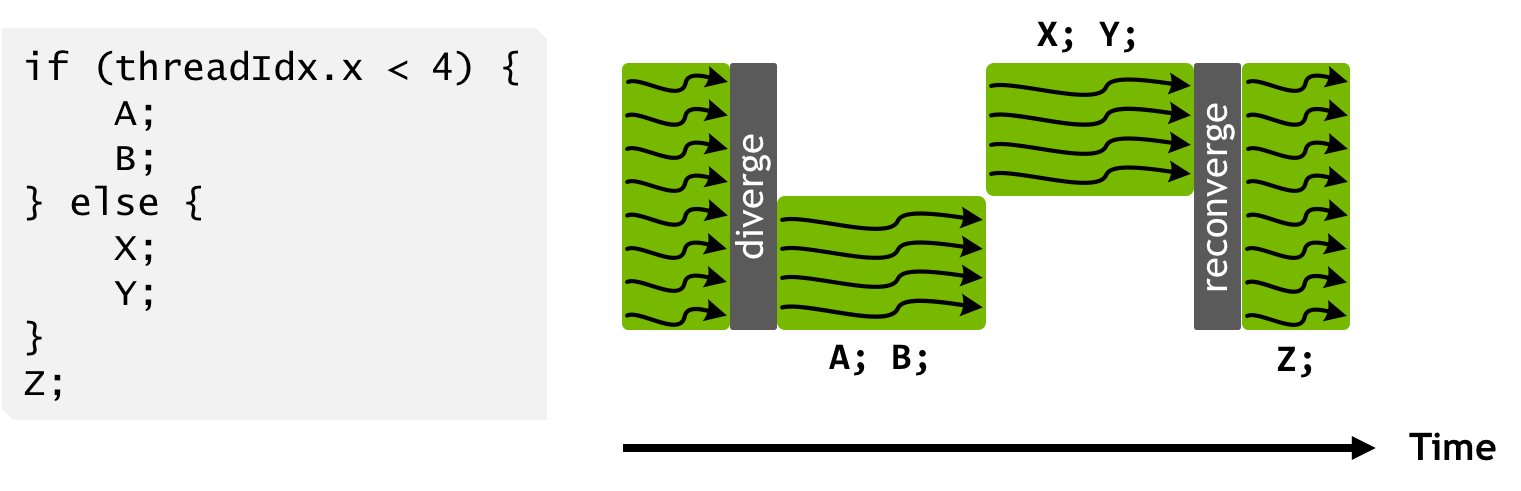
\includegraphics[width=0.8\textwidth]{cuda_thread_divergence_old.png}
	\caption{Thread divergence before Volta.}
	\label{fig:thread_divergence_old}
\end{figure}

\begin{figure}[h]
	\centering
	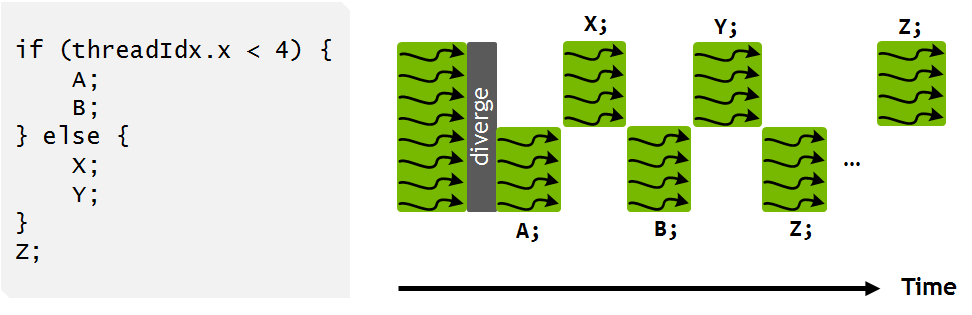
\includegraphics[width=0.8\textwidth]{cuda_thread_divergence_new.png}
	\caption{Thread divergence after Volta.}
	\label{fig:thread_divergence_new}
\end{figure}



\subsubsection{Streaming multiprocessor}
\label{sec:sm}
Processing cores in the hardware are grouped into Streaming Multiprocessors (SM). SM can be thought of as a large Vector processor with SIMD instructions which have their width hidden from the user by the SIMT model described in the section \ref{sec:simt} or by the graphics infrastructure when used by the graphics pipeline.

The diagram \ref{fig:cuda_volta_gpu} shows a single SM of the Volta Compute capability. As we can see, the SM contains integer and floating point vector units, together with the register file, schedulers, L1 instruction cache and L1 data cache and shared memory. As we can also see, these newer GPU architectures contain so called "Tensor cores", which are designed for hardware acceleration of AI. The numbers and widths of each unit may differ between different compute capabilities, which are described in the section \ref{sec:compute_capability}. These differences are again mostly hidden from the user by the SIMT model.

% TODO: Cite https://developer.nvidia.com/blog/inside-volta/
\begin{figure}[h]
	\centering
	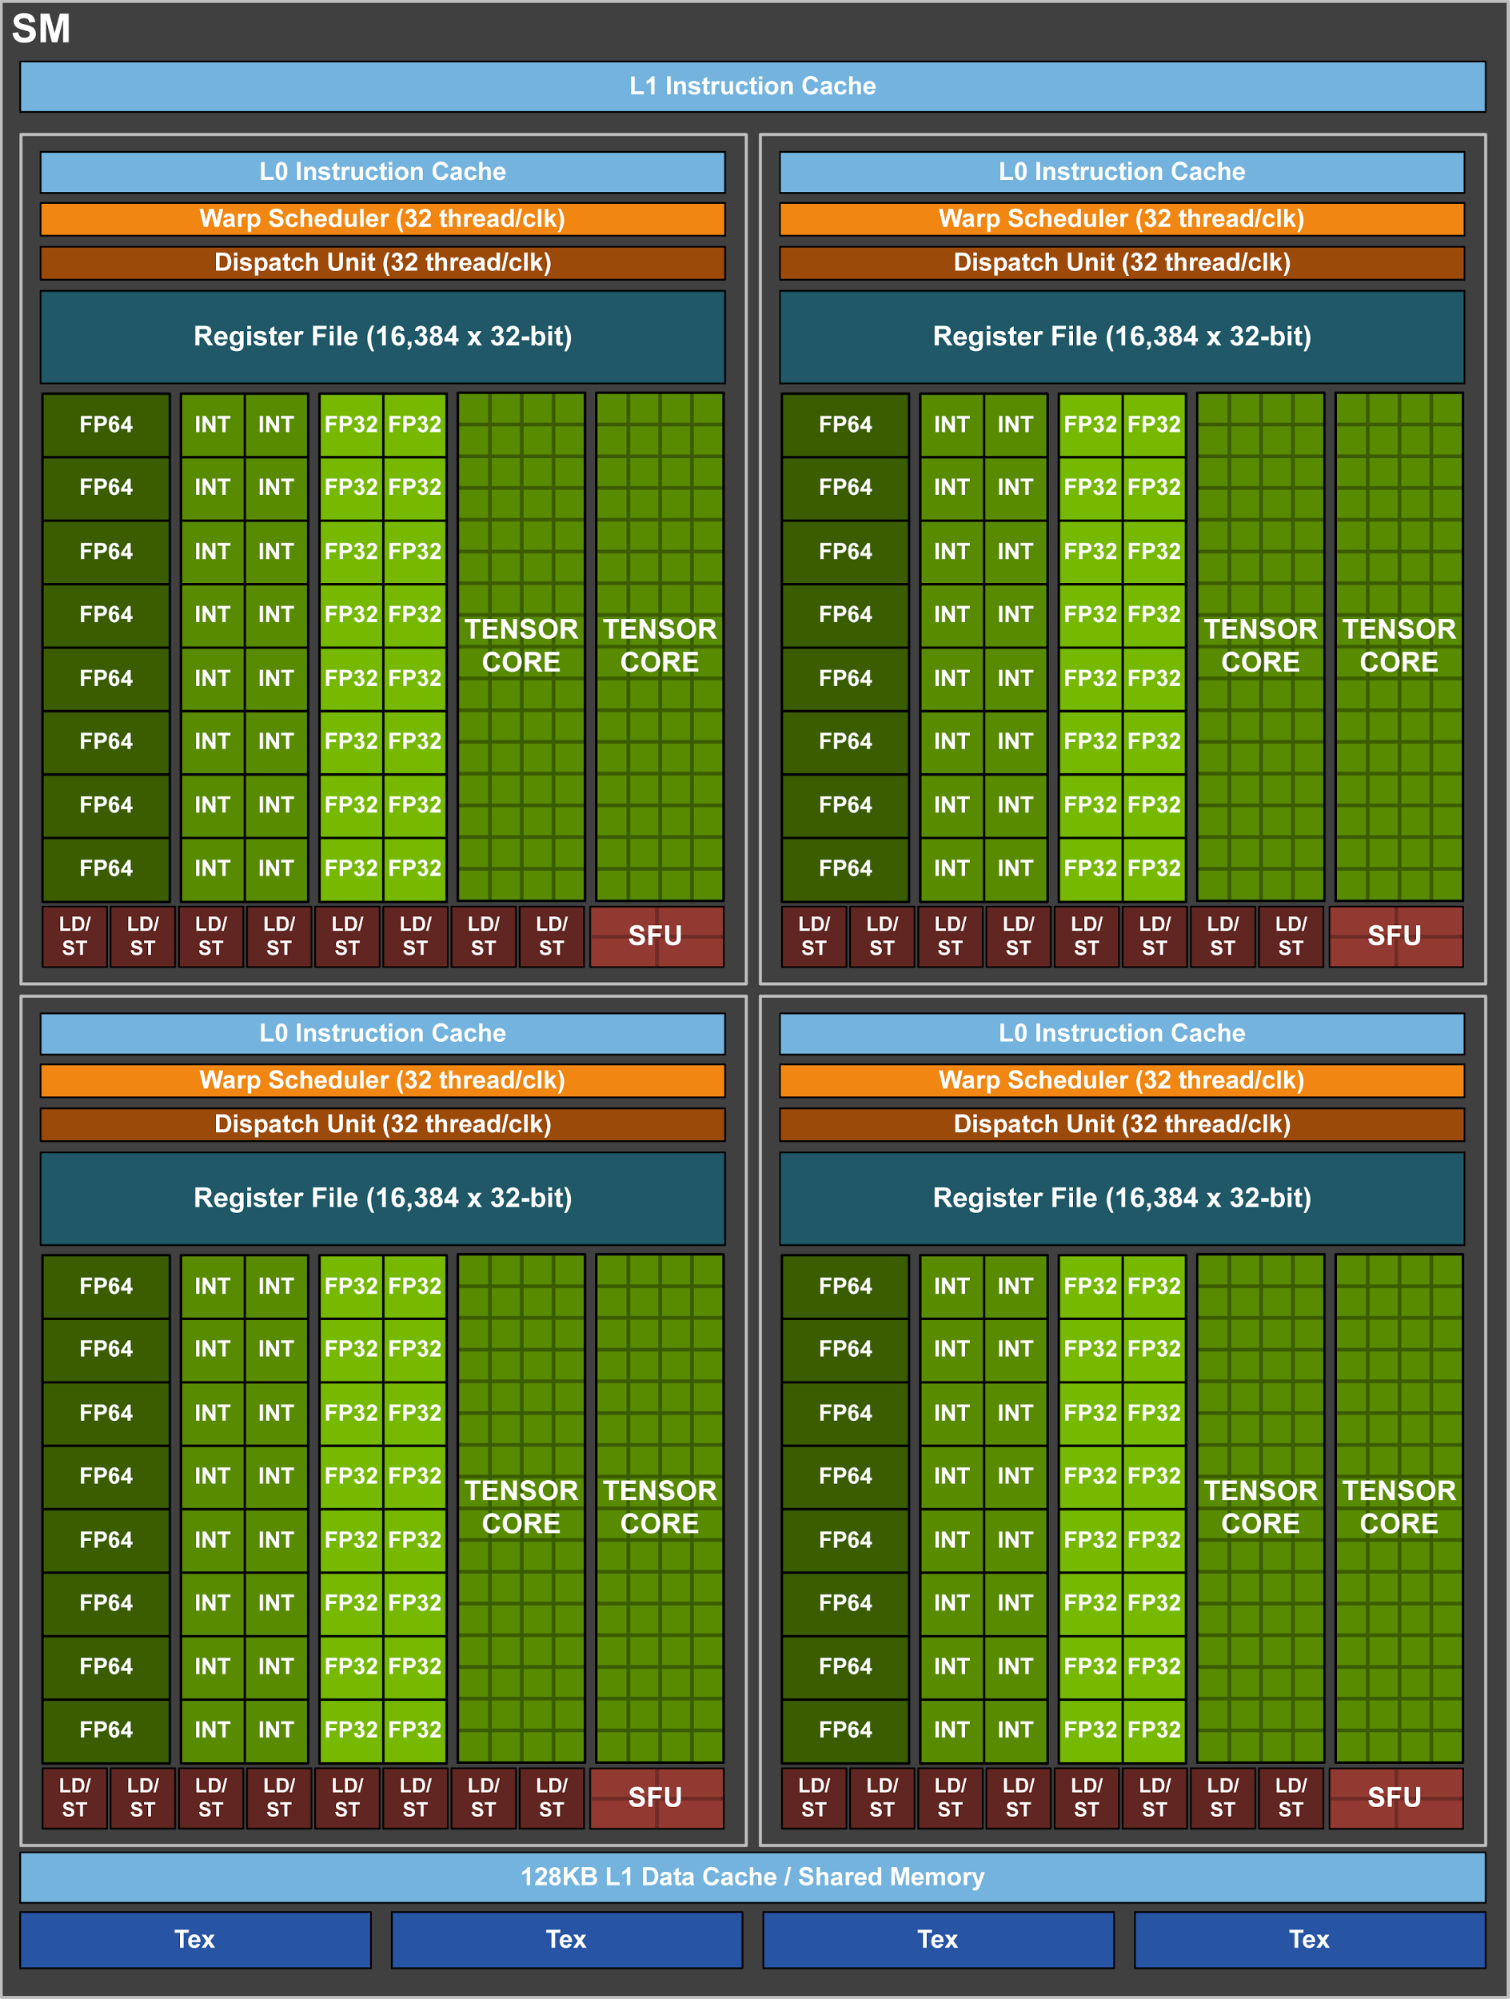
\includegraphics[width=0.8\textwidth]{volta_sm.png}
	\caption{Streaming multiprocessor of Volta GPU.}
	\label{fig:cuda_volta_gpu}
\end{figure}

Each GPU is made up of one or more SMs, which are together with the L2 cache part of the central silicon chip of the GPU. GPUs of the same Compute capability differ, among other things, mostly by the number of SMs they posses, which translates to the compute performance they can provide. 


\subsubsection{Thread hierarchy}
\label{sec:thread_hierarchy}
Threads as described in the SIMT section \ref{sec:simt}, apart from being grouped into warps for scheduling inside the Streaming multiprocessor (SM), are also grouped into Thread blocks, also called Cooperative Thread Arrays (CTA). As the name Cooperative Thread Array suggests, Thread block is a boundary for cooperation between threads. Threads in a Thread block access the same shared memory, described in section \ref{sec:memory_hierarchy}, and can easily synchronize with each other using barriers.  Whole Thread blocks are scheduled onto SM, described in section \ref{sec:sm}, completely independently and possibly in parallel, as can be seen in the figure \ref{fig:sm_scaling}. As such, threads in different Thread blocks cannot easily cooperate with each other, either through barriers or through memory. 

Whereas in the graphics pipeline each shader execution had to be independent, which allowed the shader parallelization and utilization of the whole GPU, Thread blocks are the corresponding unit of scaling in CUDA. Different GPUs of the same Compute capability, described in \ref{sec:compute_capability} differ in the number of SMs available. As we can see on the image \ref{fig:sm_scaling}, the number of SMs in a GPU determines the number of Thread blocks running in parallel and thus the total amount of time required to run the whole computation.

\begin{figure}[h]
	\centering
	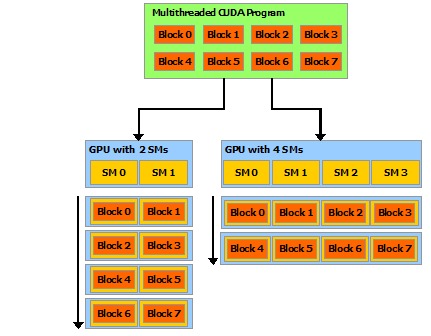
\includegraphics[width=0.8\textwidth]{cuda_sm_thread_blocks.png}
	\caption{Thread block based scaling.}
	\label{fig:sm_scaling}
\end{figure}

The limit for the number of threads in each Thread block is specific to each Compute capability. In all currently supported compute capabilities, the limit is 1024 threads. %TODO: Cite
Each thread is given unique thread ID, which is sequentially assigned scalar number. Each group of 32 threads (in current compute capabilities) with consecutive thread IDs forms a warp, described in section \ref{sec:simt}. For convenience, each thread is also assigned a thread index, which is one, two or three dimensional vector. This simplifies computations of matrices, volumes etc. Internally, the thread index is always a three dimensional vector, with the unused components zeroed out. Correspondingly, Thread blocks can be one, two or three dimensional and are internally always three dimensional with the size of unused dimensions left at 1. In the figure \ref{fig:thread_hierarchy} we can see an example of two dimensional Thread block, represented by the large yellow rectangle, with threads assigned their two dimensional indexes. The mapping between thread index and thread ID is as follows: For block of size $(D_x, D_y, D_z)$ the thread with index $(x,y,z)$ is assigned thread ID of $(x + y*D_x + z*D_x*D_y)$. This means that warp threads are consecutive in the $x$ component of the index, possibly split between consecutive values of $y$ and $z$ components if $D_x$ is not multiple of warp size.

Thread blocks are organized into a one, two or three dimensional grid of blocks as illustrated by the figure \ref{fig:thread_hierarchy}. As with threads in a block, all grids are internally three dimensional with the unused dimensions left with the size of 1. Grid is created by launching a kernel by the host code, described in \ref{sec:cuda_cpp} . The kernel launch requires two mandatory arguments, the block size and the size of the grid, specified as either a scalar number or three dimensional vector.

Newer Compute capabilities add the ability to synchronize between Thread blocks in a Grid and even between different grids, but due to the design of the GPU as described in the section \ref{sec:gpu_history}, these synchronizations have very high overhead % TODO: cite some source about the overhead
and go against the main advantage of the GPU, the massive parallelism it provides.




\begin{figure}[h]
	\centering
	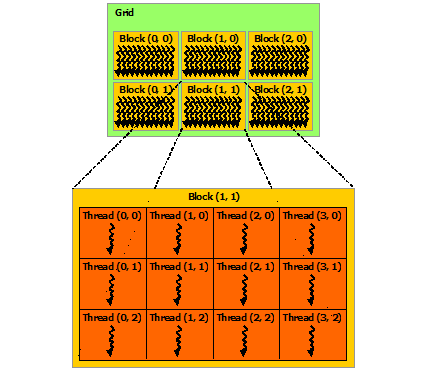
\includegraphics[width=0.8\textwidth]{grid_of_thread_blocks.png}
	\caption{Thread grouping hierarchy.}
	\label{fig:thread_hierarchy}
\end{figure}


\subsubsection{Memory hierarchy}
\label{sec:memory_hierarchy}
% TODO: Image of memory hierarchy
CUDA programming model defines several levels of memory with differing latencies and throughputs. First on the path from the host operating memory to the device processing cores is the device memory, more specifically the global memory part of the device memory. Code running on the host CPU can command the GPU driver to copy data from the host CPU memory into the global memory either directly, or create a virtual memory mapping which will automatically move the data between host operating memory and global memory using the system of memory paging. The device memory can either be present as silicon chips separate from the main GPU chip containing the Streaming multiprocessors, as can be seen in the figure \ref{fig:gpu_mem_chips}, or with the new High bandwith memory (HBM) standard, the chips seen as separate on the printed circuit board in the figure \ref{fig:gpu_mem_chips} are relocated into the central package, while still remaining separate pieces of silicon.

Apart from global memory, device memory also hosts the local, constant and texture memory. Local memory represents part of the device memory allocated for each thread used for register spilling. This is done by the compiler behind the scenes and cannot be directly controlled by the program. Constant memory contains constant values set by the host code which cannot be changed by the device code. This part of device memory is accessed through a special constant cache which aggressively caches any access to the constant values.  Last but not least there is the texture memory. Texture memory can be thought of as global memory accessed through the texture cache. It is a heritage from the graphics pipeline, used there to access textures as the name suggests. Texture memory is designed to exploit the 2D spatial locality of typical texture usage. Texture memory also provides additional features such as linear interpolation, coordinate normalization and clamping or wrapping when accessed out of bounds. As access to texture memory is only an access to global memory through caching mechanism, it is not coherent with writes to global memory within the same kernel call.




When a warp executes an instruction accessing global memory, the memory accesses of all threads of the warp are coalesced into 32, 64 or 128 byte (based on the Compute capability) naturally aligned memory transactions, depending on the addresses accessed by all the threads. For Compute capabilities 3.x and newer, the data is fetched using 32-byte transactions when cached only in L2, which is the default, or by 128-byte transactions when cached in both L1 and L2 caches. Generally if each thread accesses different 32-byte region and reads only 4 bytes from it, the total memory throughput is divided by 8 due to overfetching data that are not used in the end. Thus to maximize global memory throughput, the access of threads in a warp should be coalesced, accessing as few of the transaction blocks as possible. 

% TODO: More about access patterns to global memory, coalesced reads, writes, etc.

% TODO: Image of memory access coalescing


The L2 cache is part of the GPU chip itself, shared by all the Streaming multiprocessors. The L2 cache resembles the classic CPU caches with LRU eviction, cache lines etc. From the L2 cache, the data can optionally be cached in the L1 cache, depending on the type of data and configuration of the kernel launch. The L1 cache is local for each Streaming multiprocessor and shares hardware with the Shared memory, described in the section \ref{sec:shared_mem}. 

Finally data is copied into the register file, which is local to the Streaming multiprocessor. The size of the register file depends on the Compute capability, with the newest Ampere having 64K 32bit registers. Instructions executed by the processing cores directly use data from these registers.

% TODO: Register read after write latency


\begin{figure}[h]
	\centering
	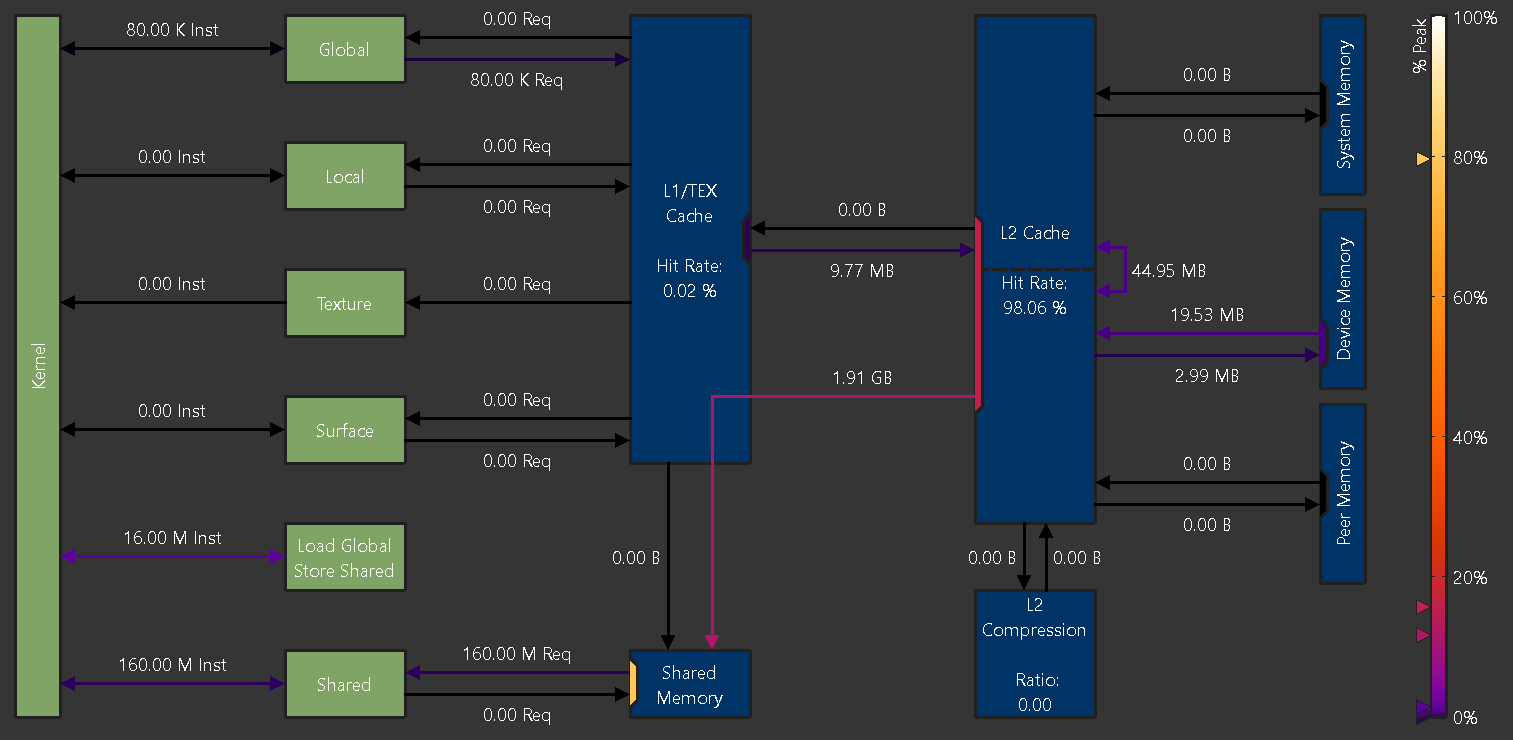
\includegraphics[width=1\textwidth]{memory_chart_a100.png}
	\caption{Types of memory in the A100 chip.}
	\label{fig:memory_chart}
\end{figure}

\begin{figure}[h]
	\centering
	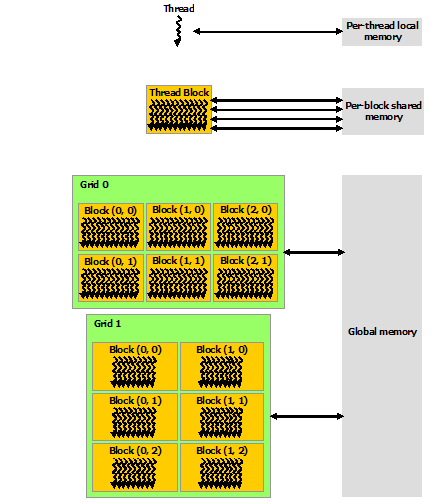
\includegraphics[width=0.8\textwidth]{cuda_memory_access.png}
	\caption{Scope of memory sharing between different groupings of threads.}
	\label{fig:memory_sharing}
\end{figure}

\subsubsection{Shared memory}

Shared memory can be described as user controlled data cache. The memory is private for the Streaming multiprocessor and is accessible and shared by all threads of each Thread block executing on the given Streaming multiprocessor. The amount of required shared memory is one of the limiting factors on the number of Thread blocks which can be scheduled onto a single SM.

Shared memory shares hardware with L1 cache, where the division of the hardware between L1 and shared memory can be configured during runtime.

In current Compute capabilities, Shared memory consists of 32 banks, where consecutive 32bit words map into consecutive banks. Each bank can handle a single request from a single thread per cycle. If two or more different addresses requested by two or more separate threads map into the same bank, these accesses will be serialized and will take two or more cycles. This situation is called bank conflict. If two or more threads access the same address, shared memory is capable of broadcasting the value to all the threads which requested the value from the given address.

Proper use of shared memory is crucial for utilizing the full throughput of the GPU.

\subsubsection{CUDA C++}
\label{sec:cuda_cpp}
CUDA platfrom, apart from defining the programming model, contains compilers, runtimes and libraries that can be used with an extension to the C++ or Fortran programming languages. As CUDA Fortran device code is also compiled by the CUDA C++ compiler, as per this thread on official nvidia forums % TODO: Add note under the line https://forums.developer.nvidia.com/t/fastest-cuda-implementation/33359/2
, we will only describe the CUDA C++ environment.

As described in the CUDA C programming guide: "CUDA C++ extends C++ by allowing the programmer to define C++ functions, called kernels, that, when called, are executed N times in parallel by N different CUDA threads, as opposed to only once like regular C++ functions. % TODO: Cite https://docs.nvidia.com/cuda/cuda-c-programming-guide/index.html#kernels

CUDA C++ adds so called "function execution space specifiers" which can be added to function declaration and have the following effect:
\begin{itemize}
	\item \_\_global\_\_ declares the function as being a kernel,
	\item \_\_device\_\_ declares the function as executed on the device, callable by another device or global function,
	\item \_\_host\_\_ declares the function as executed on the host, callable from the host only.
\end{itemize}

Without any function execution space specifier, function is compiled as if it had the \_\_host\_\_ specifier.

Kernel is a function defined using the \_\_global\_\_ declaration specifier, as described above. Kernels can be launched using the "execution configuration syntax" as shown in the snippet \ref{code:kernel_launch}.

% TODO: Example of usage of a kernel



The arguments given to the kernel launch are in the order of their specification:

\begin{enumerate}
	\item Thread block size,
	\item Grid size,
	\item Shared memory for each block in bytes,
	\item CUDA stream (described in more detail in this section).
\end{enumerate}

From these, only the Thread block size and Grid size are mandatory, the remaining two are optional.

Kernel launch is an asynchronous operation, launching the kernel and continuing the execution of host code without waiting on the kernel execution to finish.  

To identify the thread the device code, i.e. code that is executed on the device, we can use the following built-in variables:

\begin{itemize}
	\item threadIdx,
	\item blockIdx,
	\item blockDim,
	\item gridDim.
\end{itemize}

The variable threadIdx contains is a three dimensional vector with properties "x", "y" and "z" which contains the thread index, as described in \ref{sec:thread_hierarchy}. The variable blockIdx, which is also three dimensional vector, contains the index of the Thread block the current thread is part of. The blockDim variable contains the size of the Thread block, i.e. size of each of the "x", "y" and "z" dimensions of the Thread block. Lastly the gridDim variable tells us how many Thread blocks make up the current grid. These variables, mostly the first three, can be used to identify the current thread and for example read the correct part of the input, select it as the leader of the current Thread block or implement any other cooperation between the threads, as described in the section \ref{sec:thread_cooperation}.

The built-in variable "warpSize" contains the size of warp, as described in the section \ref{sec:simt}. As the value for all current Compute capabilities is 32, and "warpSIze" is a variable and not a constexpr, it is often ignored for custom constant declarations.

% TODO: Device function inlining
% TODO: CUDA Stream
% TODO: Memcpy, other CUDA API calls
% TODO: host device synchronization

\subsubsection{Thread cooperation}
\label{sec:thread_cooperation}
% TODO: Restructure this section
% 	maybe pull it into a separate subsection, something like thread cooperation

% TODO: Example code for sum or something
Threads in the device code can cooperate in many ways. Once we identify which thread we are running in using the methods described in the previous section \ref{sec:cuda_cpp}, we can also identify the threads in the same warp and the same thread block, allowing us to cooperate with these.

There exist two APIs for thread cooperation. The older one is made up of intrinsic functions, distinguishable by the "\_\_" prefix to their name, such as: \_\_syncthreads(), \_\_shfl\_* etc.
These functions allow limited granularity for synchronization and cooperation, mostly following the warp, thread block, grid granularity of the underlying abstraction. Newer API, so called "Cooperative Groups API", introduced in CUDA 9, is a superset of the older API and allows greater flexibility in groups across which threads can cooperate. 

The old API was limited to two synchronization scopes. At the scope of a Thread block, threads can cooperate by sharing data in the Shared memory and by using the intrinsic function "\_\_syncthreads()", which acts as a barrier which all threads of the Thread block must reach before any thread from the Thread block can continue beyond it. This intrinsic function also acts as a memory barrier, synchronizing accesses to memory. As per the CUDA C++ programming guide: % TODO: Cite
"the shared memory is expected to be a low-latency memory near each processor core (much like an L1 cache) and \_\_syncthreads() is expected to be lightweight".

At the scope of a warp, the old API allowed warp synchronization using the \_\_syncwarp() intrinsic function on compute capabilities newer than Volta, while also providing possibly hardware accelerated ways of sharing data between threads in the same warp using the warp shuffle functions, perform reduction-and-broadcast operations, broadcast-and-compare operations or reduction operations. For each of these warp level intrinsic functions, there is older deprecated version from before compute capability Volta without the sync suffix, which work with the implicit warp lockstep execution, and newer version with the sync suffix which implicitly syncs the warp and must be used in code compiled for compute capability Volta and newer.

Warp shuffle functions allow threads of the same warp to exchange data without the use of shared memory, moving 4 or 8 bytes of data per thread. The shuffle functions differ by which threads receive data from which threads. As of CUDA 11.5.1, there are the following warp shuffle functions:

\begin{itemize}
	\item \_\_shfl\_sync copies data from a lane with the given index,
	\item \_\_shfl\_up\_sync copies data from a lane with ID lower by given delta
	\item \_\_shfl\_down\_sync copies data from a lane with ID higher by given delta
	\item \_\_shfl\_xor\_sync copies data from based on bitwise XOR of own lane ID with given laneMask.
\end{itemize}

% TODO: Shuffle width
% TODO: No wrapping for up and down shuffle
% TODO: Wrapping for general shuffle
% TODO: Shuffle mask, all threads with bit 1 in mask must execute the shuffle
% TODO: Maybe more about shuffles, maybe leave it up to CUDA programming guide

% TODO: Warp ballot
% TODO: Warp reduce
% TODO: Warp match


The Cooperative Groups API, in addition to providing the same synchronization and cooperation tools described above, allows additional granularity for synchronization, be it across the whole grid or even multiple grids on different devices, or across subset of threads of a thread block or warp. This allows additional patterns of cooperation not possible before, such as producer-consumer pattern.

Cooperative Groups API also allows the creation of reusable code oblivious to the size of the cooperating group of threads, allowing the same code to be ran across a single warp, multiple warps of the same thread block, multiple thread blocks or the whole grid.

The API expresses the cooperating group of threads as a first class object in the device code. There are built-in function to retrieve objects for the implicit groupings of threads, be it this\_grid() for object representing the whole grid or this\_thread\_block() for an object representing the whole thread block. These objects then provide member functions to subdivide them further, returning objects representing the groups created by the subdivision.

% TODO: Example

To provide access to the warp level hardware accelerated operations, object representing thread block can be subdivided into tiled partitions of size divisible by 2 and of size smaller or equal to 32. In each thread, this call returns an object representing the warp (for size 32) or subwarp sized group the thread belongs to. This object then provides additional member methods, such as warp shuffles, warp ballots, warp sync etc.


Additionally for thread block and it's subgroups, the Cooperative Groups API provides implementation of some common functionality, such as reduce or scan operations.
% TODO: More about cooperative groups
% TODO: New memcpy async to shared memory



% TODO: Atomic operations
Atomic operations provide the means of cooperation between threads without explicit synchronization. In CUDA, these allow atomic read-modify-write operation on 32-bit or 64-bit word residing in shared or global memory. There are different classes of atomic operations based on the group of threads the operations are seen as atomic by:

\begin{itemize}
	\item System-wide (\_system suffix) are atomic across all threads in the current program, be it on other CPUs or GPUs,
	\item Device-wide (no suffix) are atomic across all CUDA threads of the current program executing on the same device as the current thread,
	\item Block-wide (\_block suffix) are atomic across all CUDA threads which belong to the same thread block as the current thread.
\end{itemize}

Compared to the atomic operations in C++ standard library, CUDA atomic operations add atomic operations over floating point data.

% TODO: Atomics do not act as memory fences

% TODO: Warp matrix functions with Tensor cores



\subsubsection{CUDA compilation}
\label{sec:cuda_compilation}
Part of the CUDA platform is the "nvcc" compiler driver. The purpose of nvcc is to separate the device code from the host code, as described in the section \ref{sec:cuda_cpp}, utilizing a general purpose C++ compiler in several compilation steps. The whole compilation process can be seen on the diagram \ref{fig:cuda_compilation}.

% TODO: Compilation in more detail
% TODO: PTX bytecode
% TODO: cubin file
% TODO: fat binary

\begin{figure}[h]
	\centering
	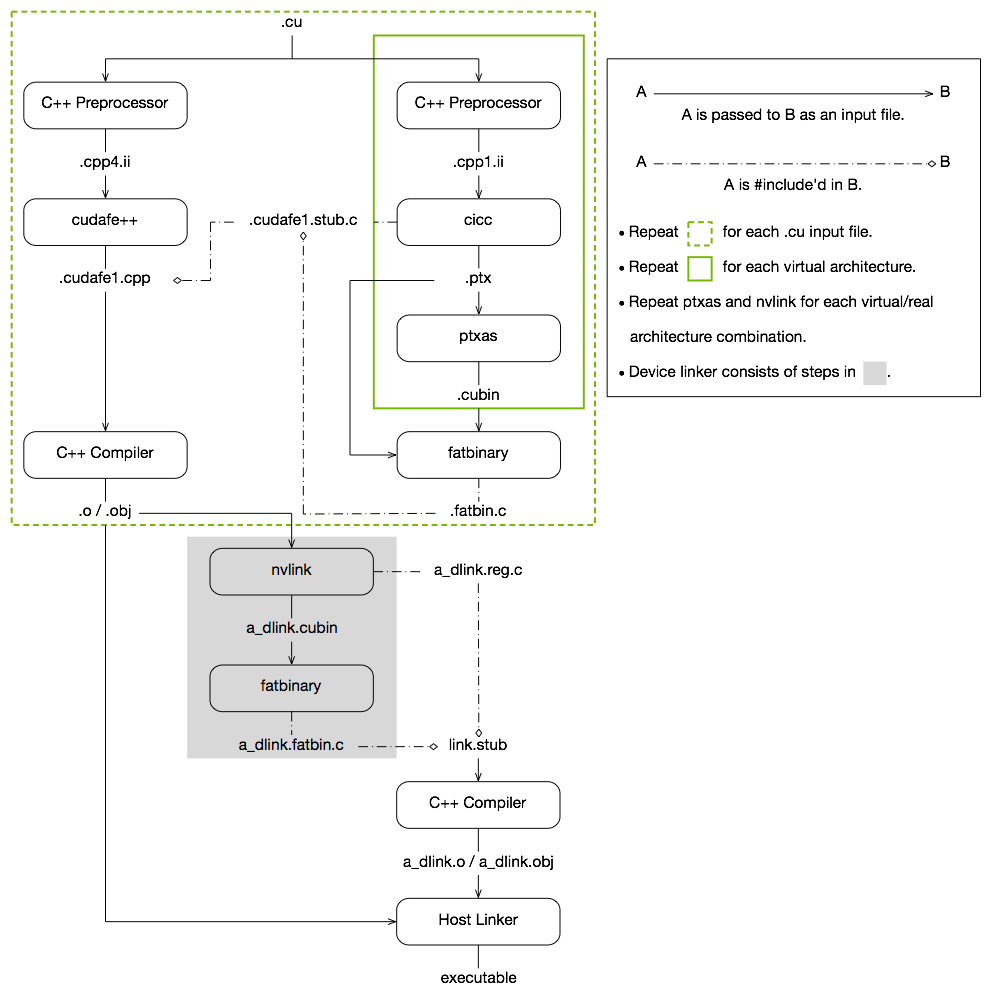
\includegraphics[width=0.8\textwidth]{cuda-compilation-from-cu-to-executable.png}
	\caption{Compilation of CUDA to binary.}
	\label{fig:cuda_compilation}
\end{figure}


\subsubsection{CUDA libraries}
\label{sec:cuda_libs}
The CUDA toolkit itself contains many libraries, implementing common problems solved using GPUs. These include cuBLAS for basic linear algebra, nvJPEG for JPEG encoding and decoding or cuSPARSE for working with sparse matrices. For our use case, the most important library provided by CUDA is the cuFFT library, implementing the Fast Fourier Transform algorithm. As described in the section \ref{sec:cross_corr_fft}, Fast Fourier transform is the most common tool used for computing cross-correlation. As there is little chance we could implement FFT faster than provided by the authors of CUDA, we will be using the FFT for the implementation using Fast Fourier transform.


